\usetikzlibrary{calc}
% Define a few constants for easy configuration
% Ensures processing of content inside a `tikzpicture` (using the short version `\tikz`)
\newcommand{\ensuretikz}{%
  \ifx\path\tikz@command@path
    \expandafter\@firstofone
  \else
    \expandafter\tikz
  \fi
}              

\def\radius{2cm}
\def\onedegrad{1.8cm}
\def\fivedegrad{1.75cm}
\def\tendegrad{1.7cm}
\def\labelrad{1.6cm}

% Define a few constants for easy configuration
              \def\radius{1.5cm}
              \def\onedegrad{1.4cm}
              \def\fivedegrad{1.25cm}
              \def\tendegrad{1.2cm}
              \def\labelrad{1.1cm}

              \newcommand\mygateway[1]{
             	\node [diamond, draw, text width=3.5em, inner sep=0pt] at (0,0) {};
              #1;
             }
           
              %CAUTION: DON'T PUT LABEL ABOVE CAPTION
              %\date{08/06/2012}
              %onlytez
              \def\mymsg{ \draw (-1.5, 1) -- ++(1.5,-1) -- ++(1.5,1);
              			  \draw (-1.5, 1) rectangle ++(3,-2);  }
              \def\myrule { 
              		\draw [very thick] (-1, 1.4) rectangle ++(2.2,-2.5); 
              	    \draw (-.7, .7) -- ++(1.6,0); 
              		\draw (-.7, .2) -- ++(1.6,0);
              		\draw (-.7, -.3) -- ++(1.6,0);}
              \def \myclock{
                \draw (0,0) circle (\radius);
                \draw[fill=black] (0,0) circle (.06mm);
              	\draw [very thick](0,3*\radius / 4) --  (0,0) -- (\radius / 2, 0);
                \node[draw, circle, inner sep=.2mm] (a) at (0,0) {};
              %  \foreach \x in {0, 6,...,360} \draw (\x:\onedegrad) -- (\x:\radius);
                \foreach \x in {0,30,...,330}
                {
                  \draw (\x:\tendegrad) -- (\x:\radius);
                };
              }              
              \newcommand \myfillesarrow  {
              \scalebox{8}{
                \node (kruispunt) at (-.29,0) {};
                \node[right of=kruispunt, node distance = .66cm]  (energieOpslag) {};
                \draw[vecArrowGreen] (kruispunt) -- (energieOpslag);
                \draw[innerGreen] (kruispunt) -- (energieOpslag);
                 }
              }        
              \newcommand\myerror{
                \node[scale=8] { $\mathcal{N} $}
              }
              \newcommand\myzabdar{ 
                \node[scale=12,very thick] { $\times $}
              }
              \newcommand\mystartevent[1]{
				\ensuretikz{
	              \draw[] (0,0) circle (2.5cm);
    	          #1;
                }
              }              
              \newcommand\myinterevent[1]{
              \ensuretikz{
              \draw[] (0,0) circle (2.5cm);
              \draw[] (0,0) circle (2cm);
              #1;
              }
              }
              \newcommand\myendevent[1]{
                        \ensuretikz{
                         \draw[fill] (0,0) circle (2.5cm);
                         \draw[fill=white] (0,0) circle (2cm);
                         #1;
                         }
                         }
               \newcommand\myterminatevent{
                                       \ensuretikz{
                                       \draw (0,0) circle (2.5cm);
                                       \draw[fill] (0,0) circle (1.4cm);
                                       }
                                       }
              \newcommand\myinnercircle{\draw [very thick](0,0) circle (2.3);}
              \newcommand\mybpmnstar{
             % \tikzstyle{scorestars}=[star] %, star points=6, star point ratio=2.25, draw,rotate=40]
                  \node[star,star points=6,fill=black,scale=7] {};
              }              
              \newcommand\mymosalas{
                \node[scale=8] { $\blacktriangleleft$\hspace{-.08cm}$\blacktriangleleft$}
              }
              \newcommand\mysubprocfork{
              	\draw (1.7,0) rectangle ++(.4,.4);	  
              	\node[scale=1.3,very thick] at (1.9\left( ,.2){ $+$}
              }
              \newcommand\mypactloop{
              \node at (2.1,-.1) (3) {};
              \path[every node/.style={very thick}] (3)   edge[loop] node  {} (3);
              }
              \newcommand\mymultiins{
              \node [very thick,scale=1] at (1.9,.2) {$||$};
              }
              \newcommand\myjoin{
              	\node at (1.5,0) (right) {};
              	\node at (.45,0) (rightcorner) {};
              		\node at (-1.5,1.5) (up) {};
              		\node at (0,.45) (upcorner) {};
              		\node at (0,-.45) (downcorner) {};
              		\node at (-1.5,-1.5) (down) {};
              	\draw [line,very thick] (rightcorner) -- (right);
              		\draw [->,draw,very thick] (up) -| (upcorner);
              			\draw [->,draw,very thick] (down) -| (downcorner);
              }
              \newcommand\mypar{
              	\node [very thick,scale=4] at (0,0) {$+$};
              }
              \newcommand\myxor{
              	\node [very thick,scale=2] at (2,1) {$Condition 1$};
              	\node [very thick,scale=2] at (0,-1) {$/$};
              	\node [very thick,scale=2] at (2,-1) {$Condition 2$};
              }

\newsavebox\bmyor
\begin{lrbox}{\bmyor}
\begin{tikzpicture}

                            	\node [very thick,scale=2] at (0,0) {};
\draw [very thick,scale=4](-.3,0) circle (.07);
                                                   	\node [very thick,scale=2] at (+1,+1) {};%\ensuremath{#1}};
                            	\node [very thick,scale=2] at (+1,-1) {};%\ensuremath{}};%#2}};
\end{tikzpicture}
\end{lrbox}
              \newcommand\myor[2]{
                            %	\node [very thick,scale=2] at (.7,.8) {\ensuremath{#1}};
                            	\draw [very thick,scale=4](0,0) circle (.07);
                            %	\node [very thick,scale=2] at (.7,-.8) {\ensuremath{#2}};
                            }

\newcommand\bpmnGatewayOr[2]{
    \mygateway{}
    \myor{#1}{#2}
}
                            
\newcommand\bmygateway[3]{
            	\node [diamond, draw, text width=3.5em, inner sep=0pt] at (#2,#3) {};
              #1;
            }

              \newcommand\myfork{
                            	\node at (-1.5,0) (left) {};
                            	\node at (-.45,0) (leftcorner) {};
                            		\node at (1.5,1.5) (up) {};
                            		\node at (0,.45) (upcorner) {};
                            		\path [<-,draw,very thick] (up) -| (upcorner);
                            		\node at (1.5,-1.5) (down) {};
                            		\node at (0,-.45) (downcorner) {};
                            	\draw [line,very thick] (left) -- (leftcorner);
                            	%	\draw [line,very thick] (upcorner) -- (up);
                            			\draw [<-,draw,very thick] (down) -| (downcorner);
                            }

              \newcommand\mybpmntask[1]{
              \ensuretikz{\draw [rounded corners] (0, 0) rectangle ++(1,.41);  
              #1;
              }
              }

\newcommand\mybpmnparjoin{
	\node [very thick,scale=3.5] at (0,0) {$+$};
	\node at (1,0) (right) {};
	\node at (.45,0) (rightcorner) {};
		\node at (0,1) (up) {};
		\node at (0,.45) (upcorner) {};
		\node at (0,-.45) (down) {};
		\node at (0,-1) (downcorner) {};
	\draw [line,very thick] (rightcorner) -- (right);
		\draw [line,very thick] (up) -- (upcorner);
			\draw [line,very thick] (downcorner) -- (down);
}


\newcommand\myerrorbpmn{
  \node[scale=10] at (2,2){ $\mathcal{N} $}
}
\usetikzlibrary{shapes.geometric,calc}
\newcommand\mybpmnzabdar{ \node[scale=18,very thick] at (2,2){ $\times$}
}
\newcommand\mybpmnmosalas{
  \node[scale=8] at (2,2){ $\blacktriangleleft$\hspace{-.08cm}$\blacktriangleleft$}
}
\newcommand\mybpmnsubprocfork{
	\draw (1.7,0) rectangle ++(.4,.4);	  
	\node[scale=1.3,very thick] at (1.9\left( ,.2){ $+$}
}
\newcommand\mybpmnpactloop{
\node at (2.1,-.1) (3) {};
\path[every node/.style={very thick}] (3)   edge[loop] node  {} (3);
}


\def \myclock{
	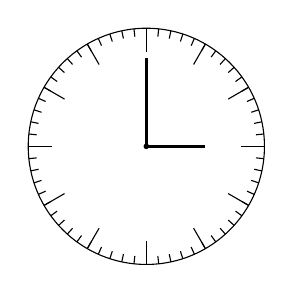
\begin{tikzpicture}[scale=1]
  % adding a subtle gray tone to add a bit of "personality"
  %\shade[shading=radial, inner color=white, outer color=gray!15] (0,0) circle (\radius);
  \draw (0,0) circle (\radius);
  \draw[fill=black] (0,0) circle (.06mm);
\draw [very thick](0,3*\radius / 4) --  (0,0) -- (\radius / 2, 0);
  \node[draw, circle, inner sep=.2mm] (a) at (0,0) {};
  % helper lines
  %\foreach \x in {0, 30, ..., 360} \draw[very thin, gray!40] (a) -- (\x:\radius);
% main lines
  \foreach \x in {0, 6,...,360} \draw (\x:\onedegrad) -- (\x:\radius);
% labels and longer lines at...but have problem with the node
  \foreach \x in {0,30,...,330}
  {
%    \node[scale=0.5] at (360-\x+90:\labelrad) {\x};
    \draw (\x:\tendegrad) -- (\x:\radius);
  };
\end{tikzpicture}          
}

\newcommand \myfillesarrowtodel  {
\scalebox{10}{
  \node (kruispunt) at (-0.145,.2) {};
  \node[right of=kruispunt, node distance = .7cm] (energieOpslag) {};
    % 1st pass
  %\draw[vecArrowWhite] (energieAanvoer) to (energieAfvoer);
  \draw[vecArrowGreen] (kruispunt) -- (energieOpslag);
 % \draw[vecArrowGreen, bend left = 30] (energieOpslag.south) to (energieAfvoer.east);
  % 2nd pass
  %\draw[innerWhite] (energieAanvoer) to (energieAfvoer);
  \draw[innerGreen] (kruispunt) -- (energieOpslag);
  %verbinding met energielevering
  %\draw[bend right=10,dotted](energieAanvoer.west) to (energieRegeling.north);
  %\draw[bend right,dotted](energieOpslag.north west) to (energieRegeling);
  %\draw[bend left=10, dotted](energieAfvoer.west) to (energieRegeling.south);
  % Note: If you have no branches, the 2nd pass is not needed
   }
}
\newcommand\myparjoin{
	\node [very thick,scale=3.5] at (0,0) {$+$};
	\node at (1,0) (right) {};
	\node at (.45,0) (rightcorner) {};
		\node at (0,1) (up) {};
		\node at (0,.45) (upcorner) {};
		\node at (0,-.45) (down) {};
		\node at (0,-1) (downcorner) {};
	\draw [line,very thick] (rightcorner) -- (right);
		\draw [line,very thick] (up) -- (upcorner);
			\draw [line,very thick] (downcorner) -- (down);
}



             
